\documentclass{article}
\usepackage{graphicx,booktabs,geometry,amsmath,enumitem}
\geometry{a4paper,margin=1in}
\title{CS4532 Concurrent Programming \\ \large Take-Home Lab 1}
\author{Fernando T.H.L (210167E) \\ Gamage M.S (210176G)}
\date{\today}
\begin{document}
\maketitle
\section*{System Information}
\noindent
\begin{minipage}[t]{0.48\textwidth}
\subsection*{CPU}
\begin{itemize}[noitemsep,topsep=0pt]
  \item Model: Intel(R) Xeon(R) Processor @ 2.30GHz
  \item Vendor/Arch: GenuineIntel / x86-64
  \item Physical cores: 4
  \item Threads per core: 1
  \item Caches:
  \begin{itemize}[noitemsep,topsep=0pt,leftmargin=*]
    \item L1i: 128 KiB (4 instances)
    \item L1d: 128 KiB (4 instances)
    \item L2:  1 MiB (4 instances)
    \item L3:  45 MiB (1 instance)
  \end{itemize}
\end{itemize}
\subsection*{Memory / NUMA}
\begin{itemize}[noitemsep,topsep=0pt]
  \item Total (kB): 8150140
  \item NUMA nodes: 1
  \item THP: madvise
  \item Swap total (kB): 0
\end{itemize}
\end{minipage}
\hfill
\begin{minipage}[t]{0.48\textwidth}
\subsection*{Operating System}
\begin{itemize}[noitemsep,topsep=0pt]
  \item Distro: Ubuntu 24.04.2 LTS
  \item Kernel: 6.8.0
  \item Logical CPUs: 4
\end{itemize}
\subsection*{Toolchain}
\begin{itemize}[noitemsep,topsep=0pt]
  \item Compiler: gcc (Ubuntu 13.3.0-6ubuntu2~24.04) 13.3.0
  \item make: GNU Make 4.3
  \item glibc: glibc 2.39
  \item libpthread (NPTL): NPTL 2.39
  \item Python: 3.12.11
  \item pandas: 2.3.2
  \item matplotlib: 3.10.6
\end{itemize}
\end{minipage}
\section*{Approach}
We implemented a singly linked list supporting:
\begin{itemize}[noitemsep,topsep=0pt]
  \item \texttt{Member}
  \item \texttt{Insert} (unique keys only)
  \item \texttt{Delete}
\end{itemize}
Three variants were tested:
\begin{itemize}[noitemsep,topsep=0pt]
  \item Serial (no locks)
  \item Pthreads + single mutex
  \item Pthreads + single read--write lock
\end{itemize}
Initialization: $n=1000$ unique keys in $[0, 2^{16}-1]$.
Workloads: $m=10000$ operations with given fractions, distributed across $T \in \{1,2,4,8\}$ threads.
Timing measures only the $m$-operations region, not initialization.
\newpage

\section*{Experiment Report (Overview Tables)}
\subsection*{Case 1: n=1000, m=10000, m\_member=0.99, m\_insert=0.005, m\_delete=0.005}
\begin{table}[h!]
\centering
\begin{tabular}{cccc}
\toprule
\textbf{Threads} & \textbf{Serial (µs)} & \textbf{Mutex (µs)} & \textbf{RW-lock (µs)} \\
\midrule
1 & 9252.00 $\pm$ 127.00 & 10112.00 $\pm$ 459.00 & 10930.00 $\pm$ 243.00 \\
2 & 9242.00 $\pm$ 75.00 & 32093.00 $\pm$ 5094.00 & 7674.00 $\pm$ 250.00 \\
4 & 8955.00 $\pm$ 288.00 & 30534.00 $\pm$ 2223.00 & 5229.00 $\pm$ 446.00 \\
8 & 8832.00 $\pm$ 212.00 & 29664.00 $\pm$ 1443.00 & 6179.00 $\pm$ 1148.00 \\
\bottomrule
\end{tabular}
\caption{Summary of results for Case 1.}
\label{tab:case1}
\end{table}
\subsection*{Case 2: n=1000, m=10000, m\_member=0.90, m\_insert=0.05, m\_delete=0.05}
\begin{table}[h!]
\centering
\begin{tabular}{cccc}
\toprule
\textbf{Threads} & \textbf{Serial (µs)} & \textbf{Mutex (µs)} & \textbf{RW-lock (µs)} \\
\midrule
1 & 17615.00 $\pm$ 825.00 & 18042.00 $\pm$ 462.00 & 29770.00 $\pm$ 533.00 \\
2 & 17107.00 $\pm$ 182.00 & 39649.00 $\pm$ 5609.00 & 30232.00 $\pm$ 908.00 \\
4 & 17372.00 $\pm$ 94.00 & 42669.00 $\pm$ 2007.00 & 22977.00 $\pm$ 823.00 \\
8 & 17664.00 $\pm$ 173.00 & 48538.00 $\pm$ 469.00 & 22568.00 $\pm$ 5037.00 \\
\bottomrule
\end{tabular}
\caption{Summary of results for Case 2.}
\label{tab:case2}
\end{table}
\subsection*{Case 3: n=1000, m=10000, m\_member=0.50, m\_insert=0.25, m\_delete=0.25}
\begin{table}[h!]
\centering
\begin{tabular}{cccc}
\toprule
\textbf{Threads} & \textbf{Serial (µs)} & \textbf{Mutex (µs)} & \textbf{RW-lock (µs)} \\
\midrule
1 & 59140.00 $\pm$ 540.00 & 61343.00 $\pm$ 512.00 & 68963.00 $\pm$ 2772.00 \\
2 & 58727.00 $\pm$ 661.00 & 85704.00 $\pm$ 6087.00 & 107904.00 $\pm$ 4267.00 \\
4 & 58024.00 $\pm$ 773.00 & 103935.00 $\pm$ 6010.00 & 120342.00 $\pm$ 4358.00 \\
8 & 57798.00 $\pm$ 1239.00 & 115380.00 $\pm$ 2375.00 & 121688.00 $\pm$ 5765.00 \\
\bottomrule
\end{tabular}
\caption{Summary of results for Case 3.}
\label{tab:case3}
\end{table}
\paragraph{Sampling/Confidence}
For Case 1, the worst relative CI was 16.29%, which exceeds the 5% target.
For Case 2, the worst relative CI was 19.56%, which exceeds the 5% target.
For Case 3, the worst relative CI was 6.23%, which exceeds the 5% target.
The target of a 5% relative CI was not met for one or more configurations, suggesting more samples are needed.
\newpage
\section*{Case Analyses with Plots}
\subsection*{Case 1: Read-Heavy Workload}
\begin{figure}[h!]
\centering
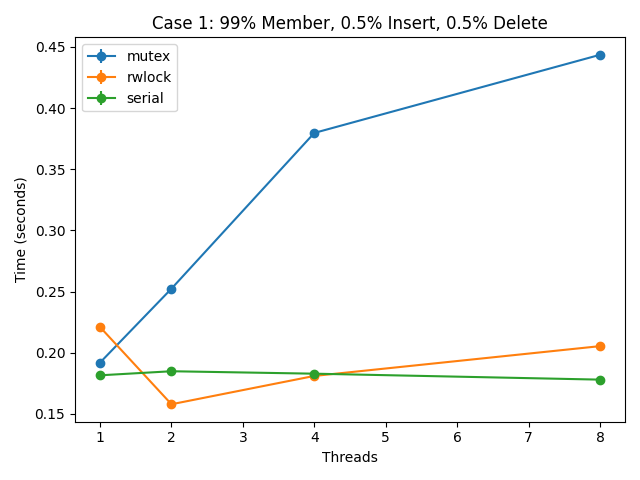
\includegraphics[width=0.9\textwidth]{report/graphs/case1_plot.png}
\caption{Average time vs. threads for Case 1.}
\label{fig:case1}
\end{figure}
\paragraph{Analysis}
As shown in Table~\ref{tab:case1} and Figure~\ref{fig:case1}, at 1 thread, serial is fastest (9252.00µs) vs mutex (10112.00µs) and rw-lock (10930.00µs).
From 1 to 8 threads, mutex changes by 193.35% and rw-lock by -43.47%.
At 8 threads, rw-lock is 4.80x faster than mutex.
This workload is read-heavy (99% member operations), which explains the significant performance advantage of the rw-lock, as it allows for concurrent reads.
\newpage
\subsection*{Case 2: Balanced Workload}
\begin{figure}[h!]
\centering
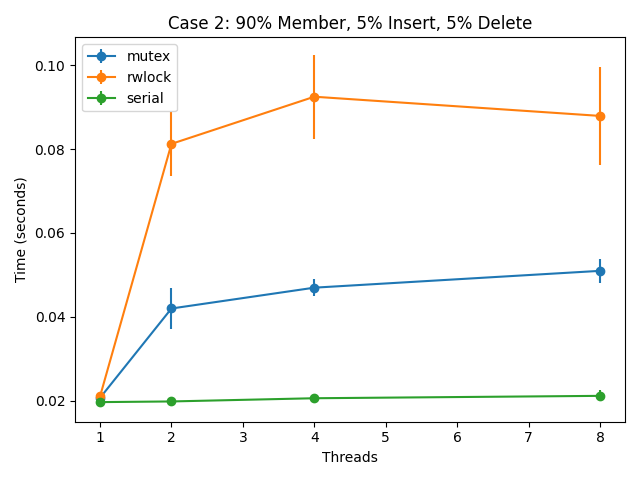
\includegraphics[width=0.9\textwidth]{report/graphs/case2_plot.png}
\caption{Average time vs. threads for Case 2.}
\label{fig:case2}
\end{figure}
\paragraph{Analysis}
As shown in Table~\ref{tab:case2} and Figure~\ref{fig:case2}, at 1 thread, serial is fastest (17615.00µs) vs mutex (18042.00µs) and rw-lock (29770.00µs).
From 1 to 8 threads, mutex changes by 169.03% and rw-lock by -24.19%.
At 8 threads, rw-lock is 2.15x faster than mutex.
With a higher write fraction (10%), the advantage of rw-lock diminishes. The data suggests that for this particular workload and system, the overhead of the rw-lock is greater than its benefit from concurrent reads.
\newpage
\subsection*{Case 3: Write-Heavy Workload}
\begin{figure}[h!]
\centering
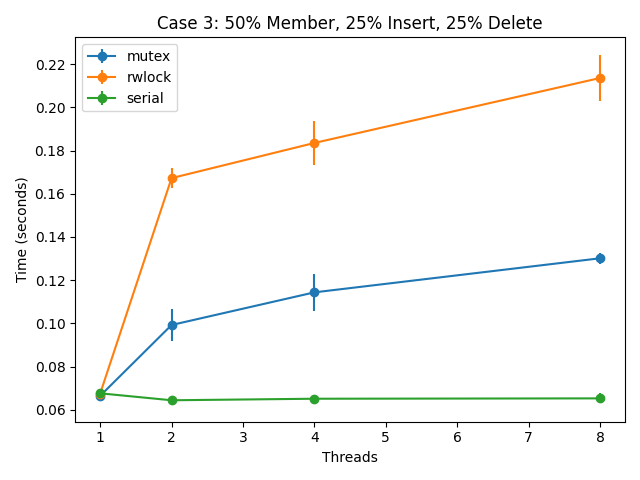
\includegraphics[width=0.9\textwidth]{report/graphs/case3_plot.png}
\caption{Average time vs. threads for Case 3.}
\label{fig:case3}
\end{figure}
\paragraph{Analysis}
As shown in Table~\ref{tab:case3} and Figure~\ref{fig:case3}, at 1 thread, serial is fastest (59140.00µs) vs mutex (61343.00µs) and rw-lock (68963.00µs).
From 1 to 8 threads, mutex changes by 88.09% and rw-lock by 76.45%.
At 8 threads, rw-lock is 0.95x faster than mutex.
In this write-heavy scenario (50% insert/delete), both locking strategies suffer from contention as writes are serialized. The rw-lock's performance is worse than the mutex, indicating that its more complex logic adds significant overhead that is not offset by parallelism in read operations.
\newpage
\begin{figure}[h!]
\centering
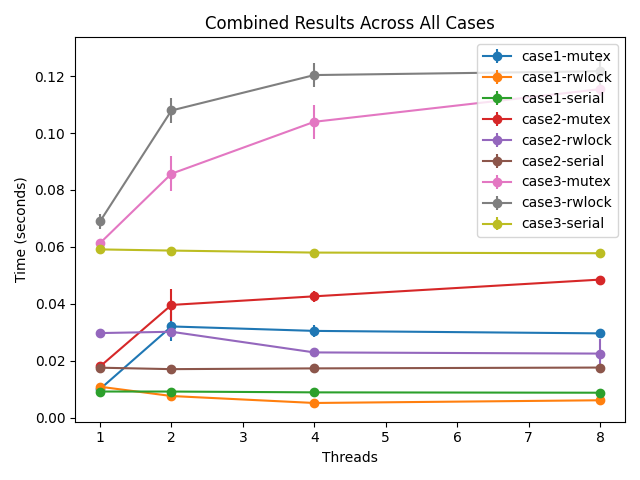
\includegraphics[width=0.8\textwidth]{{report/graphs/combined_plot.png}}
\caption{{Combined view across all cases and implementations.}}
\label{fig:combined}
\end{figure}
\section*{Conclusion}
Results align with expectations: the serial baseline dominates at T=1 (no lock overhead).
Read-heavy workloads: rwlock outperforms mutex via concurrent readers.
Write-heavier workloads: rwlock advantage shrinks; both converge due to writer serialization; parallel versions can underperform serial when contention dominates.
Scaling saturates near core count due to contention and scheduling overhead.
The $\pm$5% @ 95% CI target was not satisfied overall; it is advised to increase samples.
\end{document}